\enquestion{2.122}{
    If $P(A \mid B) = 0.6$, $P(B) = 0.8$, and $P(A) = 0.5$, are the events $A$ and $B$ independent?
}
\enanswer{
    By definition, events $A$ and $B$ are independent if $P(A \mid B) = P(A)$.
    However, $P(A) = 0.5$ and $P(A \mid B) = 0.6$, so $P(A \mid B) \neq P(A)$.
    Therefore, events $A$ and $B$ are not independent.
}

\enquestion{2.129}{
    The probability that a lab specimen contains high levels of contamination is $0.10$.
    Four samples are checked, and the samples are independent.
    \begin{enumerate}[label=(\alph*)]
        \item What is the probability that none contain high levels of contamination?
        \item What is the probability that exactly one contains high levels of contamination?
        \item What is the probability that at least one contains high levels of contamination?
    \end{enumerate}
}
\enanswer{
    As the samples are independent, we can multiply probabilities.
    Let $X$ be the number of samples with high levels of contamination.
    \begin{enumerate}[label=(\alph*)]
        \item $P(X = 0) = 0.90 \cdot 0.90 \cdot 0.90 \cdot 0.90 = 0.90^4 = 0.6561$.
        \item There are four options in this case: only the first sample is highly contaminated, only the second, only the third or only the fourth,
        each with equal probability $0.90^3 \cdot 0.10$.
        Therefore:
        \[
            P(X = 1) = 4 \cdot 0.90^3 \cdot 0.10 = 0.2916.
        \]
        \item By using the complement rule, we find:
        \[
            P(X \geq 1) = 1 - P(X \leq 0) = 1 - P(X = 0) = 1 - 0.6561 = 0.3439.
        \]
    \end{enumerate}
}

\enquestion{2.136}{
    The following circuit operates if and only if there is a path of functional devices from left to right.
    The probability that each device functions is as shown.
    Assume that the probability that a device is functional does not depend on whether or not other devices are functional.
    What is the probability that the circuit operates?
    \begin{center}
        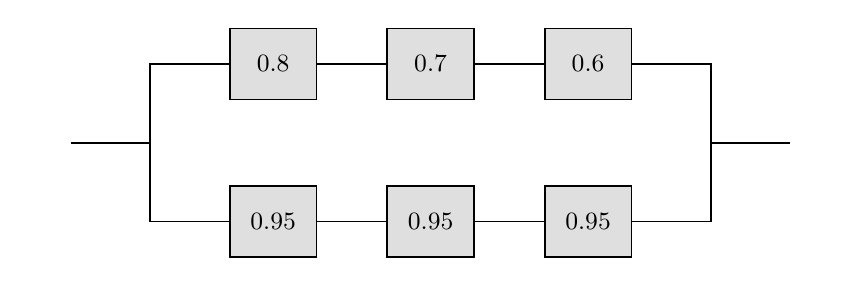
\begin{tikzpicture}[
            device/.style={draw, fill=gray!25, minimum width=1.1cm, minimum height=0.9cm, inner sep=0pt, font=\small},
            line width=0.6pt
        ]
            \node (start) at (-3, 0) {};
            \node (stop) at (7, 0) {};

            % Top branch nodes
            \node[device] (top1) at (0, 1) {0.8};
            \node[device] (top2) at (2, 1) {0.7};
            \node[device] (top3) at (4, 1) {0.6};

            % Bottom branch nodes
            \node[device] (bot1) at (0, -1) {0.95};
            \node[device] (bot2) at (2, -1) {0.95};
            \node[device] (bot3) at (4, -1) {0.95};

            % Connections inside top branch
            \draw (top1) -- (top2);
            \draw (top2) -- (top3);

            % Connections inside bottom branch
            \draw (bot1) -- (bot2);
            \draw (bot2) -- (bot3);

            % Left branching lines
            \draw (top1.west) -- ++(-1,0) -- node[midway,name=A] {} ++(0, -2) -- (bot1.west);
            \draw (A.center) -- ++(-1,0);

            % Right merging lines
            \draw (top3.east) -- ++(1,0) -- node[midway,name=B] {} ++(0, -2) -- (bot3.east);
            \draw (B.center) -- ++(1,0);

        \end{tikzpicture}
    \end{center}
}
\enanswer{
    The circuit operates if there is a path of functional devices from left to right.
    Define the events $T$ and $B$ indicating if the top or bottom line of devices all function properly.
    The probabilities $P(T)$ and $P(B)$ can be calculated as follows:
    \begin{align*}
        P(T) &= 0.8 \cdot 0.7 \cdot 0.6 = 0.336, \\
        P(B) &= 0.95 \cdot 0.95 \cdot 0.95 = 0.857375.
    \end{align*}
    We want to find the probability that either $T$ or $B$ occurs, i.e.
    \begin{align*}
        P(T \cup B) &= P(T) + P(B) - P(T \cap B) \\
                    &= P(T) + P(B) - P(T) \cdot P(B) \\
                    &= 0.336 + 0.857375 - 0.336 \cdot 0.857375 \\
                    &\approx 0.9053.
    \end{align*}
}

\enquestion{2.137}{
    The following circuit operates if and only if there is a path of functional devices from left to right.
    The probability that each device functions is as shown. 
    Assume that the probability that a device is functional does not depend on whether or not other devices are functional.
    What is the probability that the circuit operates?

    \begin{center}
        \begin{tikzpicture}[
            device/.style={draw, fill=gray!25, minimum width=1.1cm, minimum height=0.9cm, inner sep=0pt, font=\small},
            line width=0.6pt
        ]
            \node (start) at (-3, 0) {};
            \node (stop) at (7, 0) {};

            % Top branch nodes
            \node[device] (top1) at (0, 1) {0.85};
            \node[device] (top2) at (2.5, 1) {0.9};
            \node[device] (top3) at (5, 1) {0.8};

            % Bottom branch nodes
            \node[device] (bot1) at (0, -1) {0.95};
            \node[device] (bot2) at (2.5, -1) {0.75};
            \node[device] (bot3) at (5, -1) {0.9};

            \node (A) at ($(top1.center)!.5!(bot1.center)+(-1,0)$) {};
            \node (B) at ($(top1.center)!.5!(bot1.center)+(1,0)$) {};
            \node (C) at ($(top2.center)!.5!(bot2.center)+(-1,0)$) {};
            \node (D) at ($(top2.center)!.5!(bot2.center)+(1,0)$) {};
            \node (E) at ($(top3.center)!.5!(bot3.center)+(-1,0)$) {};
            \node (F) at ($(top3.center)!.5!(bot3.center)+(1,0)$) {};

            % Add connections
            \draw (top1) -| (A.center) |- (bot1);
            \draw (top1) -| (B.center) |- (bot1);
            \draw (top2) -| (C.center) |- (bot2);
            \draw (top2) -| (D.center) |- (bot2);
            \draw (top3) -| (E.center) |- (bot3);
            \draw (top3) -| (F.center) |- (bot3);

            \draw (A.center) -- ++(-1,0);
            \draw (B.center) -- (C.center);
            \draw (D.center) -- (E.center);
            \draw (F.center) -- ++(1,0);

        \end{tikzpicture}
    \end{center}
}
\enanswer{
    The circuit operates if there is a path of functional devices from left to right.
    Define the events $S_1, S_2, S_3$ indicating if either of the two parallel devices in stage $1, 2$ or $3$ function properly.
    The probabilities $P(S_1)$, $P(S_2)$ and $P(S_3)$ can be calculated as follows:
    \begin{align*}
        P(S_1) &= 1 - P(S_1') = 1 - 0.15\cdot 0.05 = 0.9925, \\
        P(S_2) &= 1 - P(S_2') = 1 - 0.1\cdot 0.25 = 0.975, \\
        P(S_3) &= 1 - P(S_3') = 1 - 0.2\cdot 0.1 = 0.98
    \end{align*}
    We want to find the probability that $S_1$, $S_2$ and $S_3$ all occur, i.e.
    \begin{align*}
        P(S_1 \cap S_2 \cap S_3)    &= P(S_1) \cdot P(S_2) \cdot P(S_3) \\
                                    &= 0.9925 \cdot 0.975 \cdot 0.98 \\
                                    &\approx 0.9483.
    \end{align*}
}

\enquestion{2.147}{
    Customers are used to evaluate preliminary product designs.
    In the past, \SI{95}{\percent} of highly successful products received good reviews, \SI{60}{\percent} of moderately successful products received good reviews,
    and \SI{10}{\percent} of poor products received good reviews.
    In addition, \SI{45}{\percent} of products have been highly successful, 
    \SI{30}{\percent} have been moderately successful, 
    and \SI{25}{\percent} have been poor products.

    \begin{enumerate}[label=(\alph*)]
        \item What is the probability that a product attains a good review?
        \item If a new design attains a good review, what is the probability that it will be a highly successful product?
        \item If a product does not attain a good review, what is the probability that it will be a highly successful product?
    \end{enumerate}
}
\enanswer{
    Let us define the following events:
    \begin{itemize}
        \item $G = \set{\text{the product has received good reviews}}$, 
        \item $H = \set{\text{the product is highly successful}}$, 
        \item $M = \set{\text{the product is moderately successful}}$,
        \item $B = \set{\text{the product is poor (bad)}}$.
    \end{itemize}
    We can derive the following probabilities from the text:

    \begin{center}
        \begin{tabular}{*{3}{c}}
            $P(G \mid H) = 0.95$ & $P(G \mid M) = 0.60$ & $P(G \mid P) = 0.10$ \\
            $P(H) = 0.45$ &  $P(M)=0.30$ & $P(B)= 0.25$
        \end{tabular}
    \end{center}

    \begin{enumerate}[label=(\alph*)]
        \item The probability that a product attains a good review is computed using the law of total probability:
        \begin{align*}
            P(G)    &= P(G \mid H) \cdot P(H) + P(G \mid M) \cdot P(M) + P(G \mid B) \cdot P(B) \\
                    &= 0.95 \cdot 0.45 + 0.60 \cdot 0.30 + 0.10 \cdot 0.25 \\
                    &= 0.6325.
        \end{align*}
        \item The probability that a product is highly successful given a good review can be computed using Bayes' Rule:
        \begin{align*}
            P(H \mid G)    &= \frac{P(G \mid H) \cdot P(H)}{P(G)} \\
                           &=\frac{0.95 \cdot 0.45}{0.6325} \\
                           &\approx 0.6759.
        \end{align*}
        \item The probability that a product is highly successful given NOT a good review can again be computed using Bayes' Rule:
        \begin{align*}
            P(H \mid G')   &= \frac{P(G' \mid H) \cdot P(H)}{P(G')} \\
                           &=\frac{(1 - 0.95) \cdot 0.45}{(1- 0.6325)} \\
                           &\approx 0.0612.
        \end{align*}
    \end{enumerate}
}

\enquestion{2.149}{
    A new analytical method to detect pollutants in water is being tested.
    This new method of chemical analysis is important because, if adopted, it could be used to detect three different contaminants --- organic pollutants, volatile solvents, and chlorinated compounds --- instead of having to use a single test for each pollutant. 
    The makers of the test claim that it can detect high levels of organic pollutants with \SI{99.7}{\percent} accuracy, volatile solvents with \SI{99.95}{\percent} accuracy, and chlorinated compounds with \SI{89.7}{\percent} accuracy. 
    If a pollutant is not present, the test does not signal.
    Samples are prepared for the calibration of the test and \SI{60}{\percent} of them are contaminated with organic pollutants, \SI{27}{\percent}
    with volatile solvents, and \SI{13}{\percent} with traces of chlorinated compounds. 
    A test sample is selected randomly.

    \begin{enumerate}[label=(\alph*)]
        \item What is the probability that the test will signal?
        \item If the test signals, what is the probability that chlorinated compounds are present?
    \end{enumerate}
}
\enanswer{
    Define the following events:
    \begin{itemize}
        \item $O = \set{\text{sample is contaminated with organic pollutants}}$,
        \item $V = \set{\text{sample is contaminated with volatile solvents}}$,
        \item $C = \set{\text{sample is contaminated with chlorinated compounds}}$,
        \item $A = \set{\text{the test signals (alarm)}}$.
    \end{itemize}
    From the text, we can derive the following probabilities:
    \begin{center}
        \begin{tabular}{*{3}{c}}
            $P(A \mid O) = 0.997$ & $P(A \mid V) = 0.9995$ & $P(A \mid C) = 0.897$ \\
            \multicolumn{3}{c}{$P(A \mid O') = P(A \mid V') = P(A \mid C') = 0$} \\
            $P(O) = 0.6$ & $P(V) = 0.27$ & $P(C) = 0.13$
        \end{tabular}
    \end{center}
    \begin{enumerate}[label=(\alph*)]
        \item The probability that the test will signal can be calculated using the law of total probability:
        \begin{align*}
            P(A)    &= P(A \mid O) \cdot P(O) +  P(A \mid V) \cdot P(V) +  P(A \mid C) \cdot P(C) \\
                    &= 0.997 \cdot 0.6 + 0.9995 \cdot 0.27 + 0.897 \cdot 0.13 \\
                    &= 0.9847.
        \end{align*}
        \item The probability that chlorinated compounds are present given a test signal can be calculated using Bayes' Rule:
        \begin{align*}
            P(C \mid A) = \frac{P(A \mid C) \cdot P(C)}{P(A)} = \frac{0.897 \cdot 0.13}{0.9847} \approx 0.1184.
        \end{align*}
    \end{enumerate}
}

\enquestion{2.154}{
    Decide whether a discrete or continuous random variable is the best model for each of the following variables:
    \begin{enumerate}[label=(\alph*)]
        \item The time until a projectile returns to earth.
        \item The number of times a transistor in a computer memory changes state in one operation.
        \item The volume of gasoline that is lost to evaporation during the filling of a gas tank.
        \item The outside diameter of a machined shaft.
        \item The number of cracks exceeding \SI{1.2}{\centi\metre} in \SI{16}{\kilo\metre} of an interstate highway.
        \item The weight of an injection-molded plastic part.
        \item The number of molecules in a sample of gas.
        \item The concentration of output from a reactor.
        \item The current in an electronic circuit.
    \end{enumerate}
}
\enanswer{
    Discrete values are those variables used for \enquote{counting} and continuous variables are used for \enquote{measuring}.
    Therefore:
    \begin{enumerate}[label=(\alph*)]
        \item continuous
        \item discrete
        \item continuous
        \item continuous
        \item discrete
        \item continuous
        \item discrete
        \item continuous
        \item continuous
    \end{enumerate}
}

\enquestion{2.180}{
    The following circuit operates if and only if there is a path of functional devices from left to right.
    Assume devices fail independently and that the probability of \textit{failure} of each device is as shown.
    What is the probability that the circuit operates?

    \begin{center}
        \begin{tikzpicture}[
            device/.style={draw, fill=gray!25, minimum width=1.1cm, minimum height=0.9cm, inner sep=0pt, font=\small},
            line width=0.6pt
        ]
            \node (start) at (-3, 0) {};
            \node (stop) at (7, 0) {};

            % Top branch nodes
            \node[device] (top1) at (0, 1) {0.01};
            \node[device] (top2) at (2, 1) {0.01};
            \node[device] (top3) at (4.5, 1) {0.01};

            % Bottom branch nodes
            \node[device] (bot1) at (1, -1) {0.1};
            \node[device] (bot2) at (4.5, -1) {0.1};

            \node (A) at ($(top1.center)+(-1,-1)$) {};
            \node (B) at ($(top2.center)+(1,-1)$) {};
            \node (C) at ($(top3.center)!.5!(bot2.center)+(-1,0)$) {};
            \node (D) at ($(top3.center)!.5!(bot2.center)+(1,0)$) {};

            % Add connections
            \draw (top1) -| (A.center) |- (bot1);
            \draw (top1) -- (top2);
            \draw (top2) -| (B.center) |- (bot1);
            \draw (top3) -| (C.center) |- (bot2);
            \draw (top3) -| (D.center) |- (bot2);

            \draw (A.center) -- ++(-1,0);
            \draw (B.center) -- (C.center);
            \draw (D.center) -- ++(1,0);

        \end{tikzpicture}
    \end{center}
}
\enanswer{
    The circuit operates if there is a path of functional devices from left to right.
    Define the events $S_1, S_2$ indicating if either the subsystems of stage $1, 2$ or $3$ function properly.
    The probabilities $P(S_1)$ and $P(S_2)$ can be calculated as follows, where we split each subsystem in a top part and a bottom part $T_i$ and $B_i$:
    \begin{align*}
        P(S_1) &= P(T_1) + P(B_1) \cdot P(T_1 \cap B_1) = \left(0.99 \cdot 0.99\right) + 0.9 - \left(0.99 \cdot 0.99 \cdot 0.9\right) = 0.99801, \\
        P(S_2) &= P(T_2) + P(B_2) \cdot P(T_2 \cap B_2) = 0.99 + 0.9 - 0.99\cdot 0.9 = 0.999.
    \end{align*}
    We want to find the probability that $S_1$, $S_2$ and $S_3$ all occur, i.e.
    \begin{align*}
        P(S_1 \cap S_2) &= P(S_1) \cdot P(S_2) \\
                        &= 0.99801 \cdot 0.999 \\
                        &\approx 0.9970.
    \end{align*}
}

\newpage

\enquestion{2.193}{
    The following circuit operates if and only if there is a path of functional devices from left to right.
    Assume that devices fail independently and that the probability of \textit{failure} of each device is as shown.
    What is the probability that the circuit does not operate?
    \begin{center}
        \begin{tikzpicture}[
            device/.style={draw, fill=gray!25, minimum width=1.1cm, minimum height=0.9cm, inner sep=0pt, font=\small},
            line width=0.6pt
        ]

            % Top parallel path
            \node[device] (top) at (3, 3) {0.02};

            % Middle-top series path
            \node[device] (midtop1) at (2, 1) {0.01};
            \node[device] (midtop2) at (4, 1) {0.1};

            % Middle-bottom series path
            \node[device] (midbot1) at (2, -1) {0.01};
            \node[device] (midbot2) at (4, -1) {0.1};

            % Bottom parallel path
            \node[device] (bot) at (3, -3) {0.02};

            % Internal connections for series branches
            \draw (midtop1) -- (midtop2);
            \draw (midbot1) -- (midbot2);


            \node (A) at ($(midtop1)+(-1,0)$) {};
            \node (B) at ($(midbot1)+(-1,0)$) {};
            \node (C) at ($(midtop2)+(1,0)$) {};
            \node (D) at ($(midbot2)+(1,0)$) {};

            % Draw lines
            \draw (top.west) -| (A.center) -- (B.center) |- (bot.west);
            \draw (top.east) -| (C.center) -- (D.center) |- (bot.east);

            \draw (midtop1.west) -- (A.center);
            \draw (midbot1.west) -- (B.center);
            \draw (midtop2.east) -- (C.center);
            \draw (midbot2.east) -- (D.center);

            \draw ($(A.center)!.5!(B.center)$) -- ++(-1,0);
            \draw ($(C.center)!.5!(D.center)$) -- ++(1,0);

        \end{tikzpicture}
    \end{center}
}
\enanswer{
    The circuit does not operate if either of the four paths fails.
    Define the events $F_1, F_2, F_3, F_4$ as either of four paths failing.
    The probabilities $P(F_1)$ up to and including $P(F_4)$ can be calculated as follows:
    \begin{align*}
        P(F_1) &= 0.02, \\
        P(F_2) &= 1 - P(F_2') = 1 - 0.99 \cdot 0.9 = 0.109, \\
        P(F_3) &= 1 - P(F_3') = 1 - 0.99 \cdot 0.9 = 0.109, \\
        P(F_4) &= 0.02.
    \end{align*}
    We want to find the probability that all four paths fail, i.e.
    \begin{align*}
        P(F_1 \cap F_2 \cap F_3 \cap F_4) &= P(F_1) \cdot P(F_2) \cdot P(F_3) \cdot P(F_4) \\
                        &= 0.02 \cdot 0.109 \cdot 0.109 \cdot 0.02 \\
                        &\approx 4.7524 \cdot 10^{-6}.
    \end{align*}
}